\documentclass[dcc]{fcfmcourse}
\usepackage{teoria}
\usepackage[utf8x]{inputenc}
\usepackage{listings}
\usepackage{mathtools}

\usepackage{hyperref}

\newenvironment{codebox} {\small \ttfamily \bgroup\obeylines} {\egroup}

\renewcommand{\figurename}{Figura.}

\setlength{\parindent}{0pt}

\title{Tarea 5: Corrector ortográfico}
\course[CC3001]{Algoritmos y Estructuras de Datos}
\professor{Nelson Baloian}
\professor{Patricio Poblete}
\assistant{Gabriel Azócar}
\assistant{Manuel Cáceres}
\assistant{Michel Llorens}
\assistant{Sergio Peñafiel}
% Si pasas el comando usedate a la clase, la fecha aparecerá bajo la lista de auxiliares.
% Puedes usar el formato de fecha pparéor defecto de latex (y traducirla usando babel)
% o puedes escribir lo que quieras con el comando \date.
% \date{1 de Septiembre, 2015}


\begin{document}
\maketitle
\vspace{-2ex}
\begin{center}
Fecha de Entrega: Miércoles 28 de Junio  \textbf{23:30hrs} \\
\end{center}


\section{Introducción}
Hoy en día la mayoría de los editores de texto, navegadores e incluso smartphones, tienen un corrector ortográfico asociado cada vez que el usuario escribe texto. Esta característica se encarga de verificar que todas las palabras escritas sean válidas en el lenguaje de entrada, si alguna es incorrecta es reportada, generalmente subrayándola en rojo. En esta tarea veremos una implementación de corrector ortográfico usando el TDA Diccionario.

\begin{figure}[!h]
    \centering
    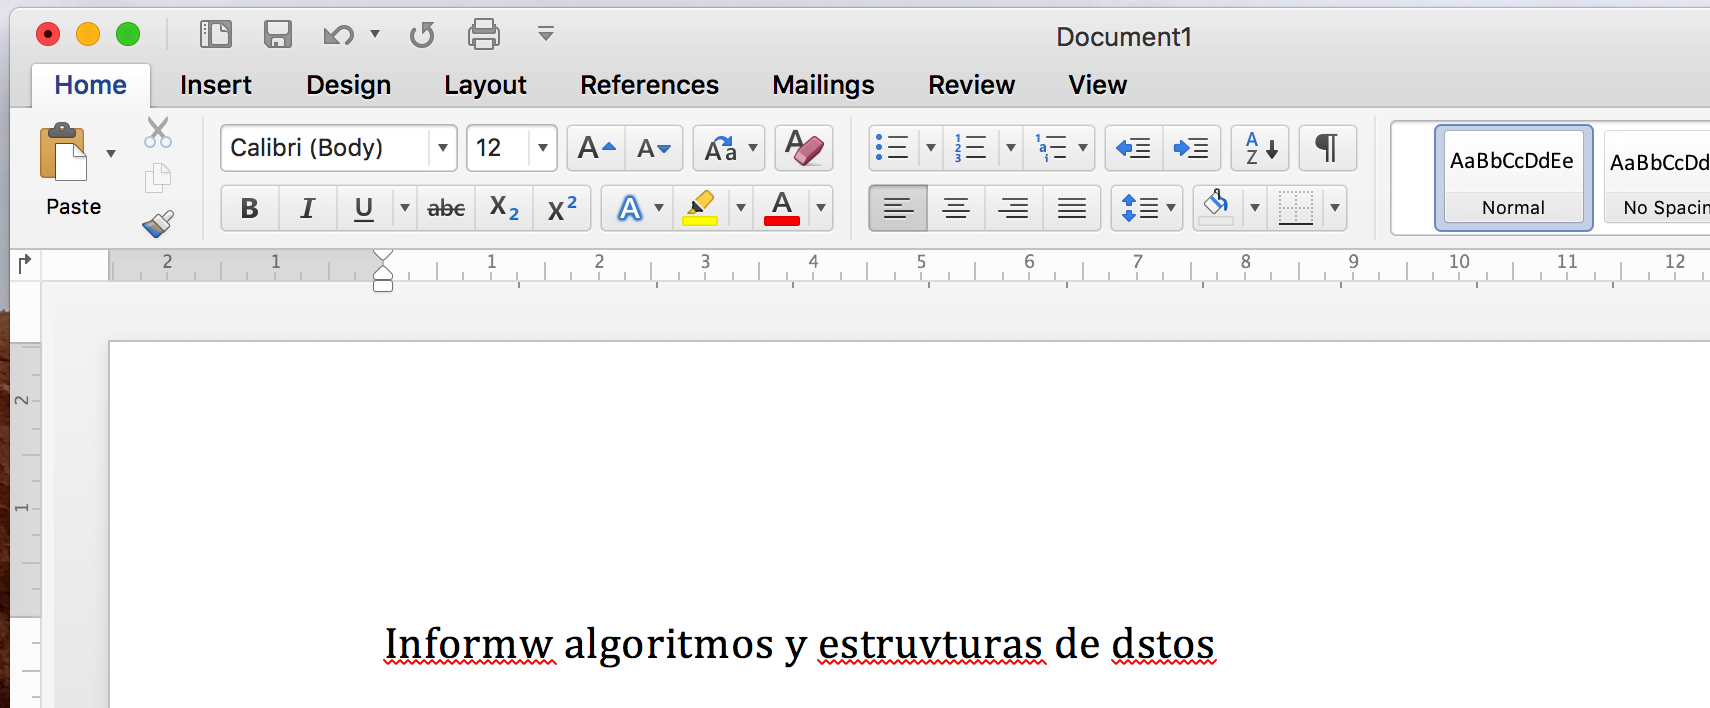
\includegraphics[scale=0.55]{imagenes/word.png}
\end{figure}

\newpage
\section{Explicación}

\subsection{TDA Diccionario}

Como se vio en clases el TDA diccionario permite asociar valores a llaves, las cuales luego se pueden recuperar. En esta tarea, usaremos una versión simplificada del TDA Diccionario, en la cual no nos importarán los valores de las llaves, sólo si existen en el diccionario o no, por lo que las  operaciones con las que cuenta son las siguiente:

\begin{enumerate}
    \item \textbf{Insertar:} Dado una llave de tipo String se inserta en el diccionario y se le asocia un valor por defecto.
    \item \textbf{Contiene:} Dado una llave retorna \texttt{true} si esta existe en el diccionario.
\end{enumerate}

\subsection{Lista de palabras}
Junto con el enunciado de esta tarea se le dará un archivo de texto con más de 174.000 palabras del idioma español. En cada línea de este archivo se encuentra una palabra distinta. Puede que esta lista no contenga todas las palabras del idioma español. \\

Se debe construir un diccionario que contenga todas las palabras del archivo entregado, para esto debe usar el TDA descrito anteriormente, leer una a una las palabras del archivo e ir agregándolas al diccionario. \\

\subsection{Corrector ortográfico}
Finalmente se pide que cree el programa principal de corrección ortográfica, este programa interactivo deberá pedir al usuario una frase (conjunto de palabras), y verificar la existencia de cada una de las palabras de la frase en el diccionario, en caso que no la contenga entonces debe ser marcada como palabra incorrecta ortográficamente.

\newpage
\section{Implementación}

En esta tarea se usarán 2 implementaciones del TDA Diccionario.

\subsection{Implementación usando AVL}
Un AVL es un árbol de búsqueda binario balanceado. Este árbol es tal que para cada nodo se cumple la siguiente propiedad:

\begin{equation*}
    |h_{izq} - h_{der}| \leq 1
\end{equation*}

Esto indica que la diferencia de alturas entre los subárboles de todos los nodos es a lo más 1.

\begin{enumerate}
    \item \textbf{Insertar:} Para insertar, primero el elemento se inserta como un ABB, se verifica si esta inserción rompe la propiedad de AVL, en caso que la rompa se realizan rotaciones simples y dobles para balancear los subarboles.
    \item \textbf{Contiene:} Para esta operación basta hacer una búsqueda normal en ABB.
\end{enumerate}

Para las comparaciones entre strings utilice el orden lexicográfico.


\subsection{Implementación usando Tries}
Un trie es una generalización de un árbol digital en la que se permite que cada nodo tenga tantos hijos como símbolos de un alfabeto. Esta estructura es muy útil para usar llaves de strings como en este caso.

\begin{enumerate}
    \item \textbf{Insertar:} Para insertar, primero se recorre el árbol hasta encontrar el prefijo más largo de la llave, luego se insertan tantos nodos como caracteres faltan para completar el string, estos se insertan tal que cada uno es hijo del anterior.
    
    \item \textbf{Contiene:} Para esta operación se debe recorrer el árbol caracter a caracter, si este camino lleva hasta una hoja entonces el diccionario contiene la palabra.
\end{enumerate}

Para almacenar los nodos hijos, cada nodo tendrá un arreglo de nodos del tamaño del alfabeto, cada índice en este arreglo representa un carácter, por lo tanto el nodo en el índice i, es el hijo del nodo actual siguiendo el camino del carácter i en el alfabeto. \\

Puede suponer que el carácter $\$$ no es parte del alfabeto. 

\subsection{Limpieza de los strings}
Se pide además que cada vez que se ingrese un string se deben realizar las siguientes operaciones de limpieza:

\begin{enumerate}
    \item Pasar todo el string a minúscula.
    \item Eliminar caracteres especiales, símbolos de puntuación y números.
\end{enumerate}

\subsection{Consideraciones}

Note que el tamaño del alfabeto es 32: 26 caracteres de A a Z, 5 vocales con tilde, y el caracter ñ. Luego para los nodos del trie puede usar arreglos de tamaño 33, dado que hay 32 caracteres admitidos más el caracter especial \$. \\

\textbf{NO} es necesario preocuparse por palabras que existan en el idioma español que no estén en la lista entregada.

\section{Ejemplos de entrada y salida}

A continuación se muestran ejemplos de entradas y salidas del programa: \\

\begin{codebox}
Frase: Un efelante se balanceaba sobre la tela de una araña
Palabras incorrectas:
efelante
\end{codebox}

\vspace{4ex}

\begin{codebox}
Frase: Corrector ortográfico
No hay palabras incorrectas
\end{codebox}

\vspace{4ex}

\begin{codebox}
Frase: compracion entre implementciones de diccionario
Palabras incorrectas:
compracion
implementciones
\end{codebox}

\vspace{4ex}

\begin{codebox}
Frase: Algoritmos y estrcturas de datos
Palabras incorrectas:
estrcturas
\end{codebox}

\newpage
\section{Informe}

El informe debe describir el trabajo realizado, la solución implementada, los resultados obtenidos
y las conclusiones o interpretaciones de estos. Principalmente debe ser breve, describiendo cada uno
de los puntos que a continuación se indican:

\begin{itemize}
    \item \textbf{Portada:} Indicando número de la tarea, fecha, autor, email, código del curso, etc.
    \item \textbf{Introducción:} Descripción breve del problema y su solución.
    \item \textbf{Análisis del problema:} Exponga en detalle el problema, los supuestos que pretende ocupar, casos de borde y brevemente la metodología usada para resolverlo.
    \item \textbf{Solución del problema:} Indique claramente los pasos que siguió para llegar a la solución
    del problema. Muestre mediante figuras y ejemplos qué es lo que realiza su código. Evite copiar todo el código fuente en el informe, sin embargo, puede mostrar las partes relevantes de éste.
    \item \textbf{Modo de uso:} Explicando brevemente cualquier dato necesario para la compilación y
    ejecución de su programa.
    \item \textbf{Resultados:} 
    \begin{enumerate}
        \item Indique, desde el punto de vista teórico, el orden de las operaciones de inserción y contiene para las 2 implementaciones del TDA, estas deben estar función de las variables: N (cantidad de llaves), P (largo de la llave a insertar/buscar), y $\sigma$ (tamaño del alfabeto).
        \item Indique el tiempo de construcción y memoria utilizada por el diccionario para cada variante.
        \item Indique el tiempo de búsqueda de N palabras para cada variante. Para esto genere una frase con N palabras (considere largos de palabra distintos) \footnote{Puede encontrar un texto de ejemplo en el siguiente link: \url{users.dcc.uchile.cl/~spenafie/el\_quijote.txt} y de éste extraer las palabras a buscar}, y realice el chequeo. Considere $N = 2^7, 2^8, \dots, 2^{17}$. Grafique los resultados obtenidos.
        \item Interprete y concluya a partir de los resultados anteriores.
    \end{enumerate}


\end{itemize}

\end{document}
